\subsection{Standard Model \ttbar+Z}
\label{sec:Bkg:ttV}

\indent ttbar produced in conjunction with a Z boson consist of about one percent of the background in the SR.  Although the background is essentially negligible we do estimate the amount of $\ttbar+\Zboson$ using a $\ttbar+\gamma$ CR. \\

\indent Using the charged leptonic $Z$ boson decays to design a CR to estimate the $\ttbar+Z$ background would produce a CR with small systematic uncertainty. However, such CR tend to have low statistics because of the small branching fraction to electrons/muons compared to the branching fraction of neutrinos.  A dilepton CR also contain a large contribution from SM ttbar and $Z$ + jets. \\

\indent We take another data driven approach by building a one-lepton CR for $\ttbar+\gamma$.  $\ttbar+\gamma$ mimics $\ttbar+Z$ as the photon is in many ways like a lighter $Z$ boson.  The CR is designed to minimize theoretical uncertainties due to the extrapolation from the $\gamma$ in CR to the $\Zboson$ in SR. \\

\indent We require exactly one signal photon and one signal lepton.  The lepton is not treated as a jet for the purpose of jet multiplicity and jet $\pt$ requirements unlike in the other one lepton CRs.  We also trigger on leptons instead of $\met$ in this region. The lepton triggers used are defined in table \ref{tb:lepTriggers}.  \\

\begin{table}[htpb]
  \caption{Single Lepton triggers}
  \begin{center}
    \begin{tabular}{c|c} \hline\hline
      Channel & Trigger \\  \hline
              & {\bf Data 2015} \\ \hline
      Electron & \verb+HLT_e24_lhmedium_L1EM20VH+  \\
      	            & \verb+HLT_e60_lhmedium+ \\
	            & \verb+HLT_e120_lhloose+         \\  
      Muon & \verb+HLT_mu20_iloose_L1MU15+ \\
      	       & \verb+HLT_mu50+ \\
      \hline
              & {\bf Data 2016} \\ \hline
      Electron & \verb+HLT_e26_lhtight_nod0_ivarloose+ \\
                     &\verb+HLT_e60_lhmedium_nod0+ \\
                     &\verb+HLT_e140_lhloose_nod0+         \\ 
      Muon & \verb+HLT_mu26_ivarmedium+ \\ 
                & \verb+HLT_mu50+ \\
      \hline \hline
    \end{tabular}
  \end{center}
  \label{tb:lepTriggers}
\end{table}


\indent We require a hight $\pt$ photon with $\pt$ greater than $150\gev$.  The high $\pt$ gamma ensures that we are in a region of phase space where the $\gamma$ $\pt$ shape will mimic the heavier $\Zboson$ $\pt$.  The true $\gamma$ $\pt$ and the $\Zboson$ $\pt$ distributions is shown in figure \ref{fig:ttZ_vs_ttGamma_pt} after selecting for a boson $\pt$ with greater then $150 \gev$.  We add a systematic uncertainty to account for the difference between the $\gamma$ and $\Zboson$ $\pt$ spectrum. \\

\begin{figure}[htpb]
\centering
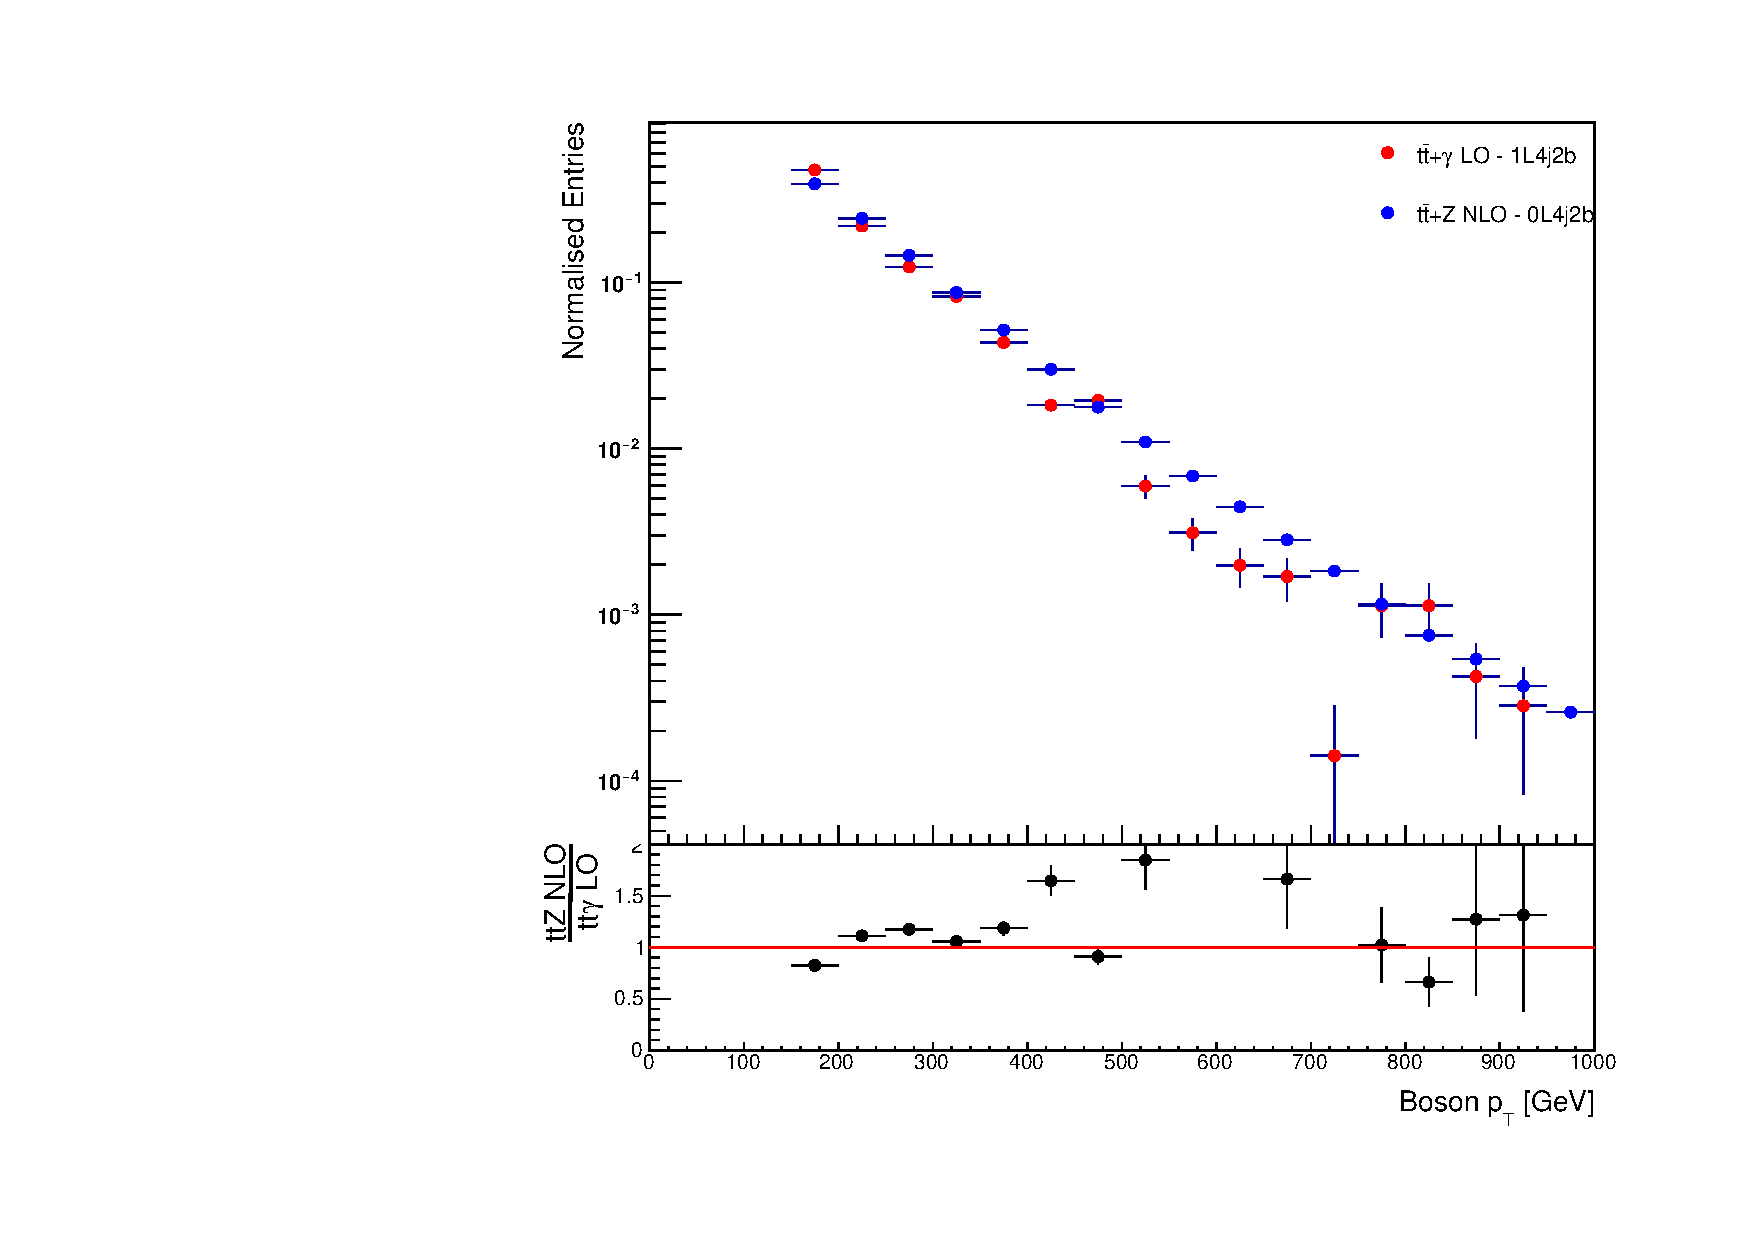
\includegraphics[scale=0.4, angle=270]{figures/ttGamma/TruthStudies/Pt150.pdf}
\caption{$\gamma$ and $\Zboson$ $\pT$ distributions with no detector resolution effects.  A selection of $\pt > 150 \gev$ has been applied.}
\label{fig:ttZ_vs_ttGamma_pt}
\end{figure}

\indent The $\ttbar+\gamma$ control region is defined in table~\ref{tb:ttG_1lepSel}.  The expected background and data yields in the $\ttbar+\gamma$ CR is given in table \ref{tb:ttVCR_2bj}. \\


\begin{table}[htpb]
  \begin{center}
    \begin{tabular}{c|c}
      \hline \hline
      Selection                 & Requirement     \\
      \hline \hline
      Event selection & Event cleaning \\
      \hline
       Trigger  & 1L Triggers  \\  \hline
      Leptons & $= 1$ \\
      Lepton \pt & 28 $\GeV$ \\
      \hline
      Photons & exactly 1\\
      \hline
      jet multiplicity & $ \ge 4 $ \\
      \hline
      Jet \pT\ & (80,80,40,40) GeV \\
      \hline
      b-jet multiplicity & $\ge 2$ \\
      \hline
      $\gamma$ \pT\ & $> 150$ GeV \\
      \hline\hline
    \end{tabular}
  \end{center}
    \caption{Selection for the $\ttbar+\gamma$ one lepton CR. The one lepton triggers as described in Table~\ref{tb:lepTriggers}}
      \label{tb:ttG_1lepSel}
\end{table}


\begin{table}[htpb]
  \caption{Background composition of $t\bar{t}\gamma$ CR.}
  \begin{center}
\begin{tabular}{c|c}
\hline\hline
\multicolumn{2}{c}{\bf CRTTGamma (87\% purity)} \\ \hline 
ttGamma & 112.20 $\pm$ 1.49 \\
VGamma & 6.41 $\pm$ 0.70 \\
Z & 0.73 $\pm$ 0.21 \\
dibosons & 0.00 $\pm$ 0.00 \\
ttbar & 4.57 $\pm$ 1.23 \\
singleTop & 2.01 $\pm$ 0.81 \\
ttV & 2.42 $\pm$ 0.28 \\
W & 0.04 $\pm$ 0.02 \\
\hline
Total MC & 128.38 $\pm$ 2.23 \\
Data & 160.00 $\pm$ 12.65 \\
 \hline
SF & 1.28 $\pm$ 0.12 \\
\hline\hline
\end{tabular}

    
  \end{center}
  \label{tb:ttVCR_2bj}
\end{table}

\indent Kinematic distributions in the $\ttbar+\gamma$ control region are shown in figure ~\ref{fig:ttgamma}  The MC background has been normalized to data by performing a simultaneous fit to all CRs.  The hashed bands on the total SM background correspond to the total experimental systematical uncertainty plus the MC statistical uncertainty.   \\

\begin{figure}[htbp]
\begin{center}
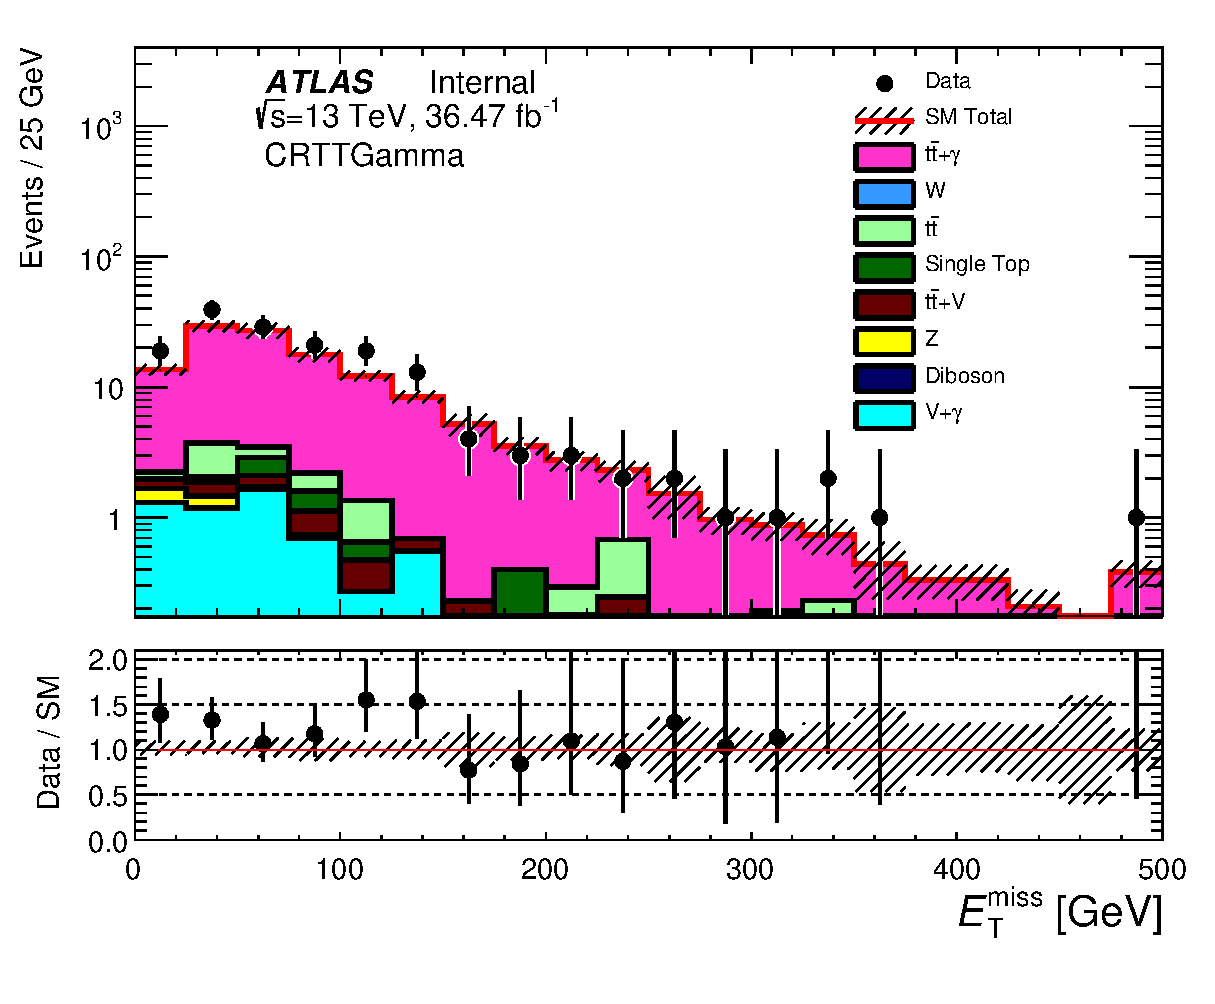
\includegraphics[width=0.49\textwidth]{figures/ttGamma/Met_CRTTGamma_withRatio_log.eps}
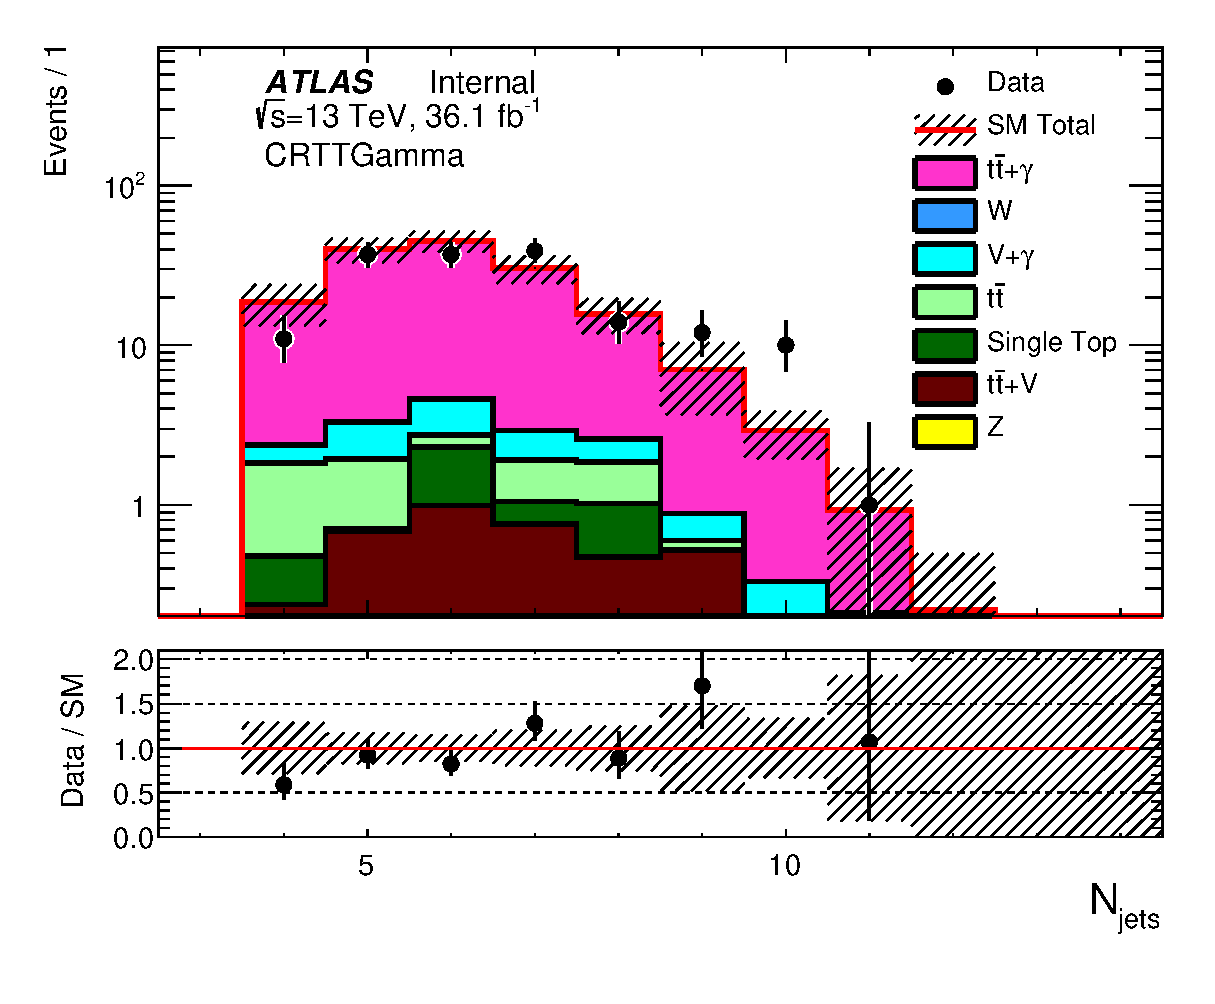
\includegraphics[width=0.49\textwidth]{figures/ttGamma/postfit/NJets_CRTTGamma_log.eps}
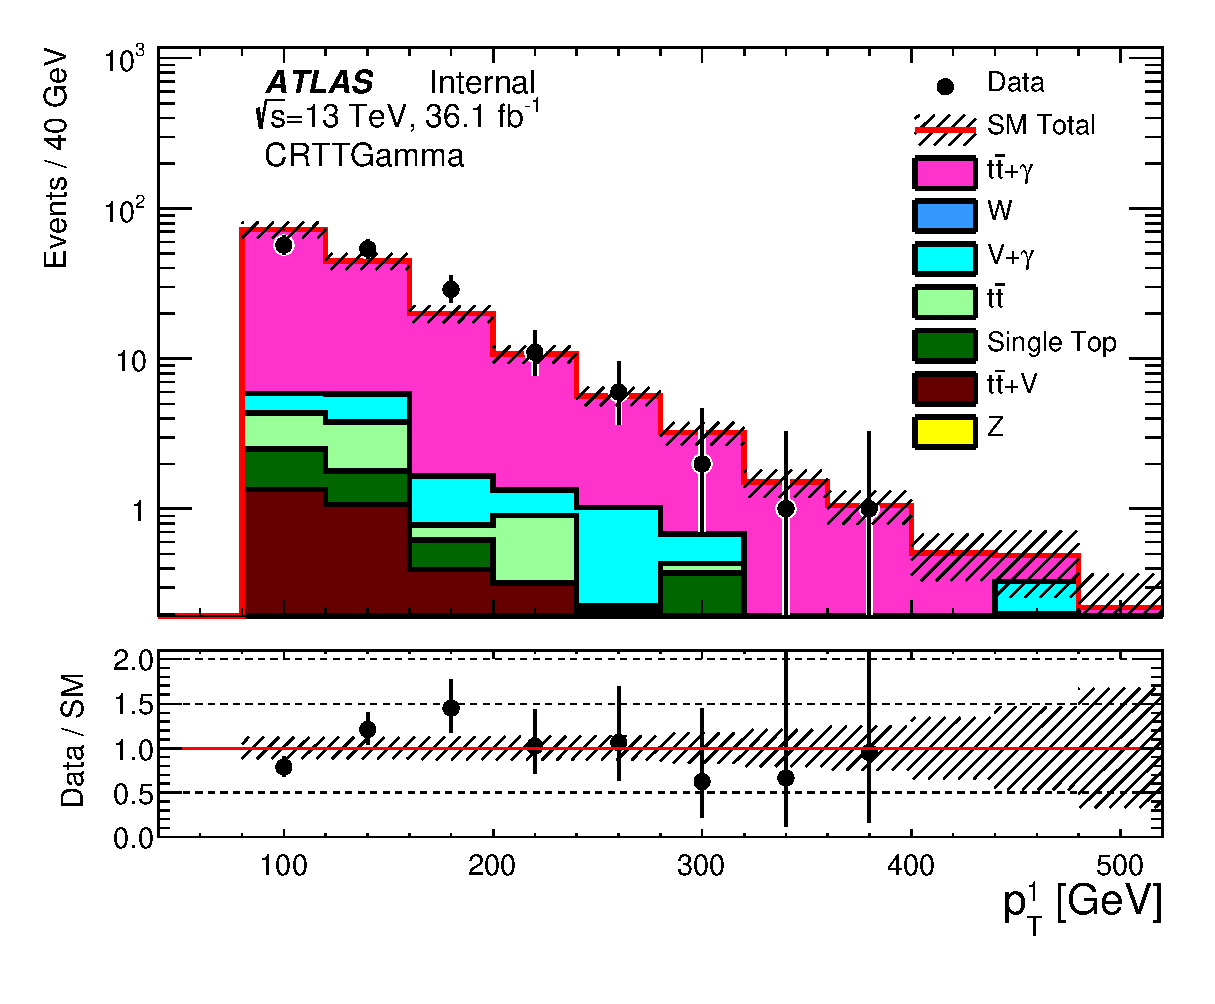
\includegraphics[width=0.49\textwidth]{figures/ttGamma/postfit/JetPt_1__CRTTGamma_log.eps}
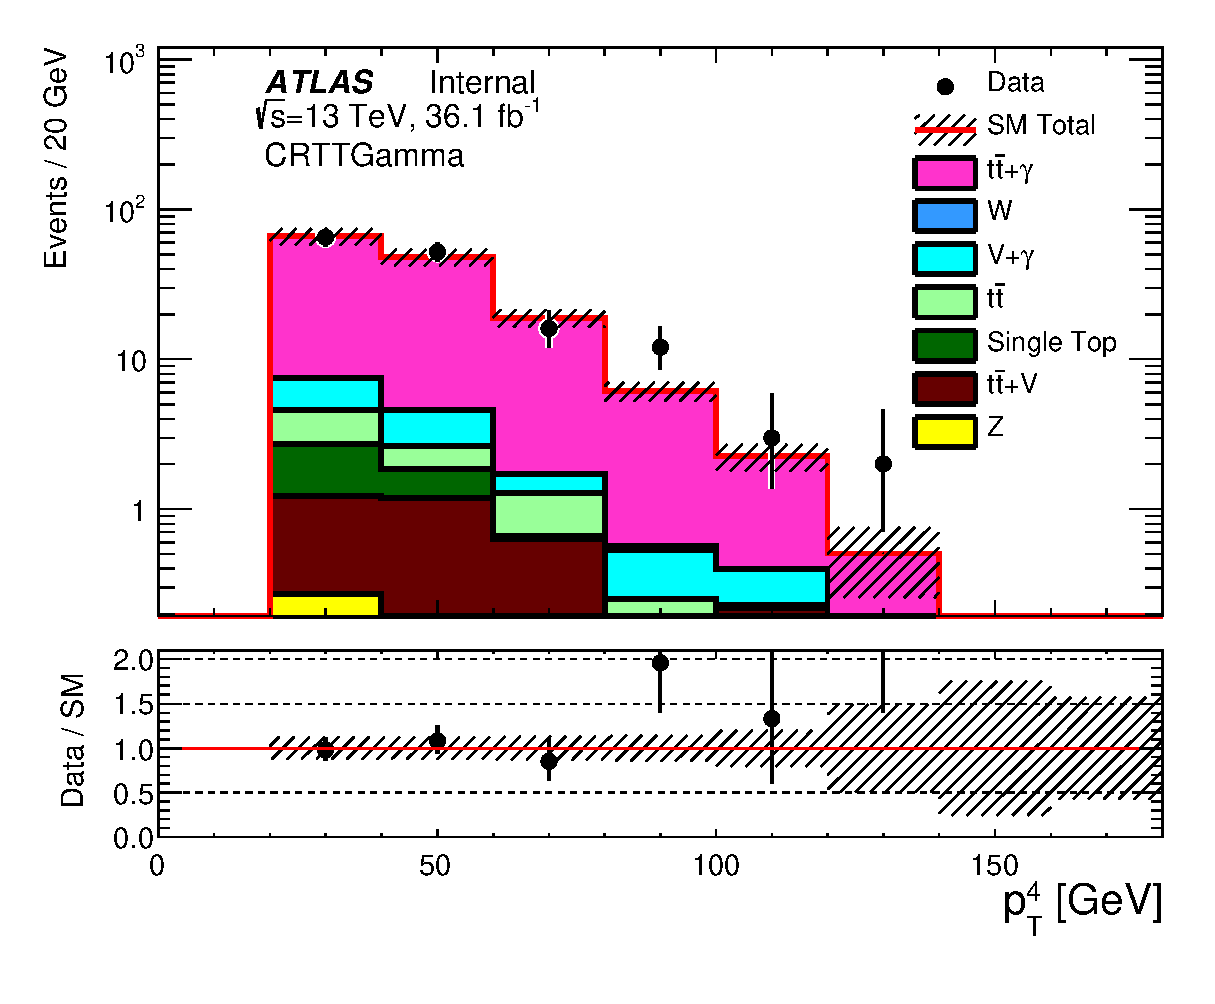
\includegraphics[width=0.49\textwidth]{figures/ttGamma/postfit/JetPt_4__CRTTGamma_log.eps}
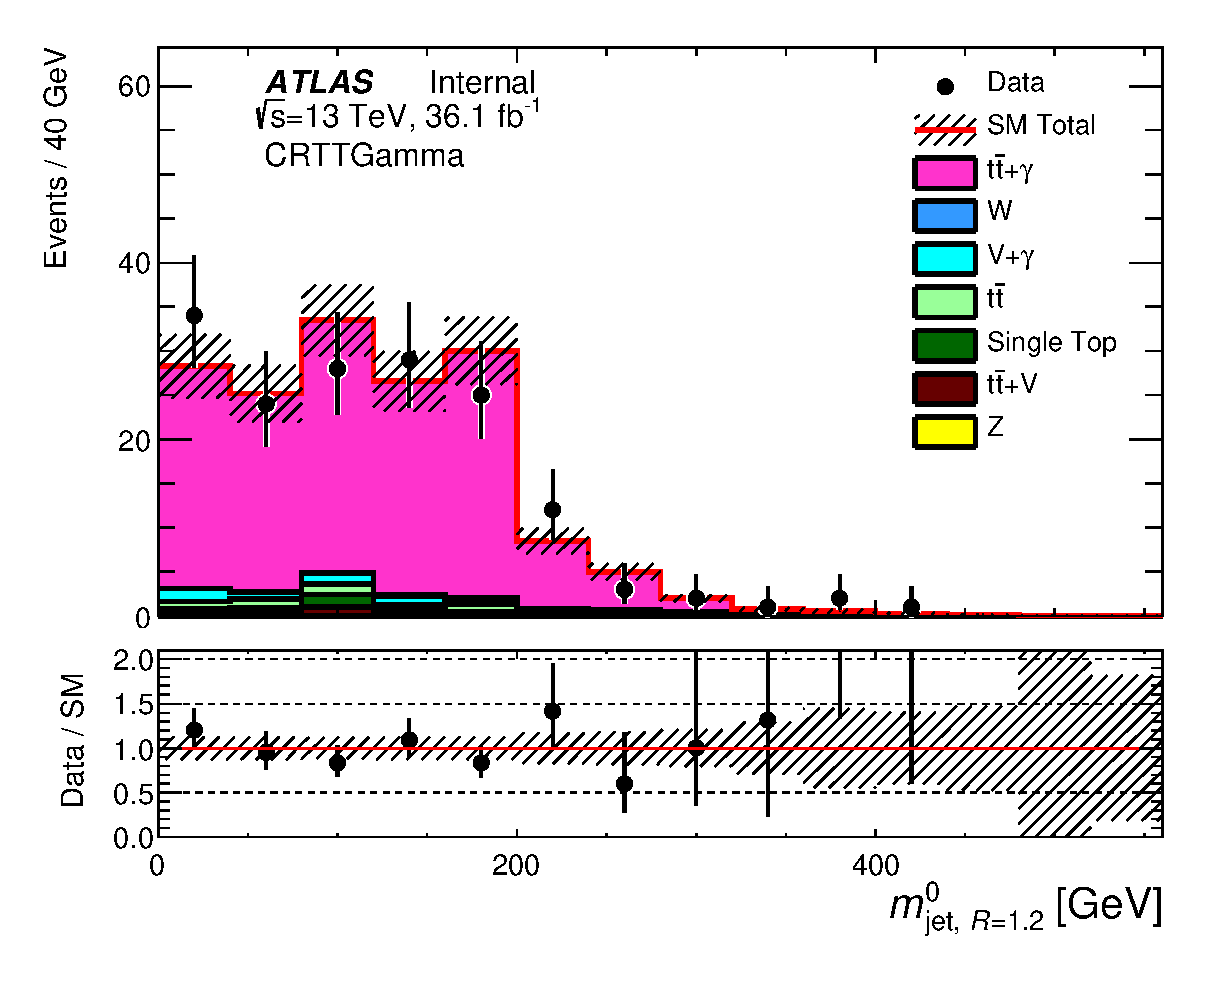
\includegraphics[width=0.49\textwidth]{figures/ttGamma/postfit/AntiKt12M_0__CRTTGamma.eps}
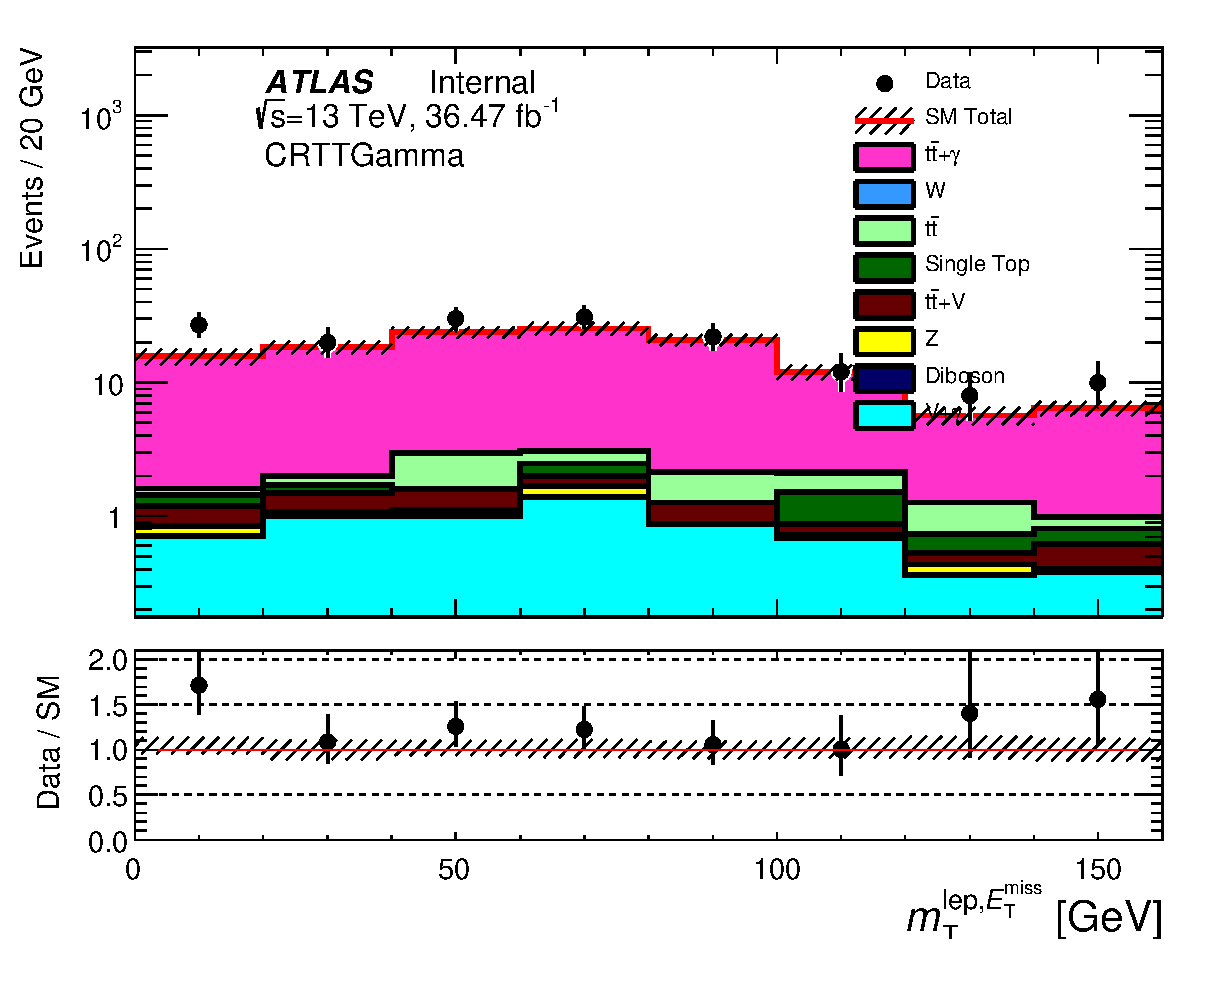
\includegraphics[width=0.49\textwidth]{figures/ttGamma/MtMetLep_CRTTGamma_withRatio_log.eps}
\caption{\label{fig:ttgamma} Distributions of select kinematic variables in the $\ttbar+\gamma$ CR. The hashed area in both the top and lower panel represents the uncertainty due to MC statistics.}
\label{fig:ttgamma}
\end{center}
\end{figure}





